%%%%%%%%%%%%%%%%%%%%%%%%%%%%%%%%%%%%%%%%%%%%%%%%%%%%%%%%%%%%%%%%%%%%%%
% Lớp 10 | Phương pháp tọa độ trong mặt phẳng (𝑂𝑥𝑦) | Ba đường conic trong mặt phẳng tọa độ
% Dạng 0H9?5-0: Bài toán tổng hợp/thực tế, PP tọa độ hóa 3 đường conic
% Số câu: 8  (sinh tự động bởi tach_cau.py; từ nay thầy sửa trực tiếp file này)
%%%%%%%%%%%%%%%%%%%%%%%%%%%%%%%%%%%%%%%%%%%%%%%%%%%%%%%%%%%%%%%%%%%%%%

%%%%%%%%%%%%%%%% ĐÚNG/SAI %%%%%%%%%%%%%%%%

% nguồn: MaHoaNH_DungSai_Lop10
\begin{ex}%[0H9H5-0]%[ma:f7fa27cc]
	Xác định tính đúng sai của các khẳng định  sau?
	\choiceTF 
		{$\dfrac{x^2}{5}+\dfrac{y^2}{4}=1$ có tiêu cự bằng $1$} 
		{\True $\dfrac{x^2}{7}-\dfrac{y^2}{10}=1$ có hai  tiêu điểm là $F_1(-\sqrt{17};0)$, $F_2(\sqrt{17};0)$}
		{\True $y^2=18x$ có đường  chuẩn $x+\dfrac{9}{2}=0$}
		{\True$y^2=18x$ có tiêu điểm $F\left( \dfrac{9}{2};0\right)$} 
	 \loigiai{
		\begin{itemchoice}
			 \itemch \textbf{Sai}.\\
			 Ta có $\dfrac{x^2}{5}+\dfrac{y^2}{4}=$ là phương trình chính tắc của đường elip với $\heva{&a=\sqrt{5}\\& b=2}\Rightarrow c^2=a^2-b^2=1$.\\
			Do đó tiêu cự  $2c=2$.
			\itemch \textbf{Đúng}.\\ 
			Ta có $\dfrac{x^2}{7}-\dfrac{y^2}{10}=1$ là phương trình  chính tắc của hypebol với $\heva{&a=7\\&b=\sqrt{10}.}$\\
			Suy ra $c^2=a^2+b^2=17\Rightarrow c=\sqrt{17}$.\\ 
			Do đó hai tiêu điểm là  $F_1\left(-\sqrt{17};0\right)$, $F_2\left(\sqrt{17};0\right)$.
			\itemch  \textbf{Đúng}.\\
			$y^2=18x$ là phương trình chính tắc của parabol với $p=9$. Vậy đường chuẩn là $x+\dfrac{9}{2}=0$. 
			\itemch  \textbf{Đúng}.\\
			$y^2=18x$ là phương  trình chính tắc của parabol với $p=9$. Vậy tiêu điểm $F\left( \dfrac{9}{2};0\right)$.
		\end{itemchoice}
	} 
\end{ex}


%%%%%%%%%%%%%%%% TRẢ LỜI NGẮN %%%%%%%%%%%%%%%%

% nguồn: MaHoaNH_TraLoiNgan_Lop10
\begin{bt}%[0H9H5-0]%[ma:f3531db0]
	Một nhà mái vòm chứa máy bay có mặt cắt nửa hình elip cao $10 \, \mathrm{m}$ rộng  $24 \, \mathrm{m}$. Tính khoảng cách theo phương thẳng đứng từ một điểm cách chân tường $4 \, \mathrm{m}$ đến nóc nhà vòm (Làm tròn đến 2 chữ số thập phân).
	\begin{center}
		\begin{tikzpicture}[scale=0.5,font=\footnotesize,line join=round,line cap=round,>=stealth]
				 \draw[green!50!black] (8,0) arc (0:180:8 and 7.8);
				\foreach \i in  {1,2,3,4,5,6,7,8,9,10,11}
				\draw[green!50!black] (0,0)--({15*(\i)}:8 and 7.8); 
				\fill[draw=green!50!black,white] (7.6,0) arc (0:180:7.6  and 7.5)--cycle;
				\draw[green!50!black] (7.6,0) arc (0:180:7.6  and 7.5);
				\draw[green!50!black] (6.7,0.8) arc (0:180:6.7 and  6.3);
				\foreach \i in {1,2,3,4,5,6,7,8,9,10,11} 
				\draw[green!50!black] (0,0.8)--($(0,0.8)+({15*(\i)}:6.7 and  6.3)$);
				\fill[draw=green!50!black,white] (6.4,0.8) arc  (0:180:6.4 and 6.1)--cycle;
				 \draw[green!50!black] (6.4,0.8) arc (0:180:6.4 and 6.1);
				\draw[green!50!black] (5.4,1.6) arc  (0:180:5.4 and 4.8);
				\foreach \i in {1,2,3,4,5,6,7,8,9,10,11} 
				\draw[green!50!black] (0,1.6)--($(0,1.6)+({15*(\i)}:5.4  and 4.8)$);
				\fill[draw=green!50!black,white] (5.15,1.6) arc (0:180:5.15  and 4.6)--cycle;
				\draw[green!50!black] (5.15,1.6) arc  (0:180:5.15 and 4.6);
				\foreach \i  in {1,2,3,4,5,6,7,8}
				\draw[green!50!black] (0,3.5)--({20*(\i)}:8  and 7.8);
				 \fill[draw=green!50!black,white] (4.1,2.4) arc (0:180:4.1 and 3.3)--cycle;
				\draw[green!50!black] (4.1,2.4) arc (0:180:4.1 and 3.3); 
				 \foreach \i in {1,2,3,4,5,6,7,8,9,10,11}
				\draw[green!50!black] (0,2.4)--($(0,2.4)+({15*(\i)}:4.1 and 3.3)$); 
				\fill[draw=green!50!black,white] (3.85,2.4) arc (0:180:3.85 and 3.1)--cycle; 
				\draw[green!50!black]  (3.85,2.4) arc (0:180:3.85 and 3.1);
				\fill[middle color=cyan,opacity=0.05] (8,0) arc  (0:180:8 and 7.8);
				\fill[draw=green!50!black,bottom color=cyan!20!white,top color=white]  (3.85,2.4) arc (0:180:3.85 and 3.1)--cycle;
				\draw[color=green!50!black] ($(0,2.4)+(60:3.85 and  3.1)$)|-(0,2.4) coordinate[pos=0.1](A);
				 \draw[color=green!50!black] ($(0,2.4)+(120:3.85 and 3.1)$)|-(0,2.4) coordinate[pos=0.1](B);
				\draw[color=green!50!black] ($(0,2.4)+(60:3.85 and 3.1)$)|-($(0,2.4)+(30:3.85  and 3.1)$)
					($(0,2.4)+(120:3.85 and 3.1)$)|-($(0,2.4)+(150:3.85 and 3.1)$) 
					 (A)--(B);
				 \fill[bottom color=gray!40!white,top color=white] (8,0)--(4.1,2.4)--(-4.1,2.4)--(-8,0)--cycle;
				\fill[color=black] (1,1.4)--(1.5,0.9)--++(0.1,0)--(1.1,1.4)--cycle; 
				 \fill[color=black] (1.5,0.8)--++(0,0.7)--++(0.1,0)--++(0,-0.7)--++(0.3,0)--++(0,-0.5)--++(-0.2,0)--++(0,0.4)--++(-0.3,0)--++(0,-0.4)--++(-0.2,0)--++(0,0.5)--++(0.3,0)--cycle;
				 \fill[left color=gray] (2.6,1) circle (0.5 cm);
				\fill[right color=black] (2.6,1)  circle (0.4 cm);
				 \fill[left color=gray] (3.7,1.23) circle (0.4 cm);
				 \fill[right color=black] (3.7,1.23) circle (0.3 cm);
				\fill[xscale=-1,color=black]  (1,1.4)--(1.5,0.9)--++(0.1,0)--(1.1,1.4)--cycle;
				 \fill[xscale=-1,color=black] (1.5,0.8)--++(0,0.7)--++(0.1,0)--++(0,-0.7)--++(0.3,0)--++(0,-0.5)--++(-0.2,0)--++(0,0.4)--++(-0.3,0)--++(0,-0.4)--++(-0.2,0)--++(0,0.5)--++(0.3,0)--cycle;
				\fill[xscale=-1,left color=gray] (2.6,1) circle (0.5  cm);
				 \fill[xscale=-1,right color=black] (2.6,1) circle (0.4 cm);
				\fill[xscale=-1,left  color=gray] (3.7,1.23) circle (0.4 cm);
				\fill[xscale=-1,right color=black]  (3.7,1.23) circle (0.3 cm);
				\fill[left color=gray,right  color=cyan!50!black] (0.75,1.5)--(6,1.9)--++(0.5,0.35)--++(-0.2,0)--(6,2)--(0.7,1.9)--cycle;
				\fill[left color=yellow!40!white,right color=cyan!50!black]  (0.75,1.5)--(6,1.9)--($(0,1.3)+(-5:0.8 and 0.5)$) arc (0:-94:0.75 and 0.4)--($(0,1.5)+(-90:0.75 and 0.5)$) arc (-90:0:0.75 and 0.5)--cycle;
				\fill[xscale=-1,right color=gray,left color=cyan!50!black]  (0.75,1.5)--(6,1.9)--++(0.5,0.35)--++(-0.2,0)--(6,2)--(0.7,1.9)--cycle;
				\fill[xscale=-1,right color=yellow!40!white,left color=cyan!50!black]  (0.75,1.5)--(6,1.9)--($(0,1.3)+(-5:0.8 and 0.5)$) arc (0:-94:0.75 and 0.4)--($(0,1.5)+(-90:0.75 and 0.5)$) arc (-90:0:0.75 and 0.5)--cycle;
				\fill[left  color=gray,right color=cyan!50!black] (0.7,2)--(3.1,2.15)--++(0.05,0.05)--($(0,2)+(15:0.7 and 0.5)$)--cycle;
				\fill[xscale=-1,right color=gray,left color=cyan!50!black] (0.7,2)--(3.1,2.15)--++(0.05,0.05)--($(0,2)+(15:0.7 and  0.5)$)--cycle;
				\fill[bottom  color=yellow!40!white,top color=cyan!40!black] ($(0,2)+(80:0.7 and 0.5)$)--(0,5)--($(0,2)+(100:0.7 and 0.5)$)--cycle;
				\fill[bottom color=black!70,top color=cyan] (0.7,2) arc  (0:180:0.7 and 0.5)--(-0.75,1.5) arc (180:0:0.75 and 0.2)--cycle;
				\fill[top color=black!70,bottom color=cyan!50!white](-0.75,1.5) arc (-180:0:0.75 and 0.5) arc  (0:180:0.75 and 0.2)--cycle;
				\fill[color=black] (0.75,1.5)--(0.7,2)--(0,1.9)--(-0.7,2)--(-0.75,1.5) arc (180:0:0.75 and 0.2)--cycle; 
				\fill[pattern color=gray,pattern=vertical  lines] (0.75,1.5)--(0.7,2)--(0,1.9)--(-0.7,2)--(-0.75,1.5) arc (180:0:0.75 and 0.2)--cycle;
				\fill[color=black] ($(0,1.3)+(-90:0.75 and  0.4)$)--(0.1,0.6)--++(0.1,0)--++(0,-0.3)--++(-0.1,0)--++(0,0.25)--($(0,1.25)+(-90:0.75 and 0.4)$)--cycle;
				\fill[xscale=-1,color=black]  ($(0,1.3)+(-90:0.75 and 0.4)$)--(0.1,0.6)--++(0.1,0)--++(0,-0.3)--++(-0.1,0)--++(0,0.25)--($(0,1.25)+(-90:0.75 and 0.4)$)--cycle;
			\end{tikzpicture}
	\end{center}
	 \shortans{7,45}
	\loigiai{ 
		Ta đặt hệ trục tọa  độ như sau:\\
		\begin{center}
			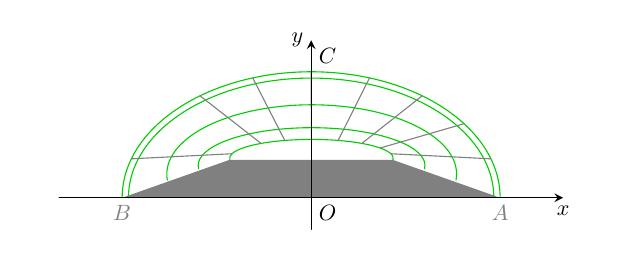
\begin{tikzpicture}[line join=round,line cap=round,scale=.8,transform shape,>=stealth]
					\clip  (-4.5,-.5) rectangle (4.5,2.7);
					 \def\xmin{-4} \def\xmax{4}
					\def\ymin{-.5}  \def\ymax{2.5}
					\draw  (-3,0)--(3,0);
					\draw[color=green!80!black] (2.9,0) arc (0:180:2.9 cm and 1.9cm); 
					\draw[color=green!80!black] (2.3,0.28) arc (-5:185:2.3  cm and 1.1cm);
					\draw[color=green!80!black] (1.8,0.46) arc  (-5:185:1.8 cm and 0.6cm);
					\fill[gray](-1.3,0.6)--(1.3,0.6)--(3,0) node[below]{$A$}--(-3,0) node[below]{$B$}--cycle; 
					 \draw[color=green!80!black] (3,0) arc (0:180:3 cm and 2cm) coordinate[pos=0.1] (A) coordinate[pos=0.2] (C) coordinate[pos=0.3] (E) coordinate[pos=0.4] (G) coordinate[pos=0.5] (I) coordinate[pos=0.6] (M) coordinate[pos=0.7] (P) coordinate[pos=0.8] (T) coordinate[pos=0.9] (L);
					\draw[color=green!80!black] (1.3,0.6) arc (-5:185:1.3 cm and 0.3cm) coordinate[pos=0.1] (B) coordinate[pos=0.2] (D) coordinate[pos=0.3] (F)  coordinate[pos=0.4] (H) coordinate[pos=0.5] (J) coordinate[pos=0.6] (N) coordinate[pos=0.7] (Q) coordinate[pos=0.8] (K) coordinate[pos=0.9] (Z);
					\draw[color=gray]  (A)--(B)
						(C)--(D) 
						(E)--(F) 
						(G)--(H) 
						(I)--(J) 
						(M)--(N) 
						(P)--(Q) 
						 (L)--(Z);
					\draw[->]  (\xmin,0)--(\xmax,0) node [below]{$x$};
					\draw[->] (0,\ymin)--(0,\ymax)  node [left]{$y$};
					\node at (0,0)  [below right]{$O$};
					\node  at (0,2) [above right]{$C$};
				\end{tikzpicture}
		\end{center}
		$AB$ là độ dài trục  lớn của elip nên $2a=24\Leftrightarrow a=12$, $OC$ là một nửa trục bé nên $b=10$.\\
		Vậy phương  trình của elip có hình mái vòm là $\dfrac{x^2}{144}+\dfrac{y^2}{100}=1$.\\
		Gọi điểm $D$ là điểm cách chân tường  $4 \mathrm{m}$ khi đó khoảng cách từ $D$ đến gốc tọa độ là $8 \mathrm{m}$.\\
		Vậy ta có $D(8;y_D)$ thỏa mãn  phương trình elip nên $\dfrac{{{8}^{2}}}{144}+\dfrac{y_{D}^{2}}{100}=1\Leftrightarrow \left| {{y}_{D}} \right|=\dfrac{10\sqrt{5}}{3}$.\\
		Vậy khoảng cách theo phương thẳng đứng từ  điểm $D$ đến nóc là $\left| y_D \right|\approx 7,45$.
	 }
\end{bt}

% nguồn: MaHoaNH_TraLoiNgan_Lop10
\begin{bt}%[0H9V5-0]%[ma:53ea331b]
	Ta biết rằng mặt trăng chuyển động quanh trái đất theo quỹ đạo là một elip mà trái đất là một tiêu điểm. Elip có chiều dài trục lớn và trục nhỏ lần lượt là $769\,266$ (km) và $768\,106$ (km). Tính khoảng cách ngắn nhất từ trái đất đến mặt trăng (đơn vị $10^3$ km), biết  rằng cách khoảng cách đó đạt được khi trái đất và mặt trăng nằm trên trục lớn của elip.
	 \shortans{364}
	\begin{center}
		\begin{tikzpicture}[scale=1,font=\footnotesize,line join=round,line cap=round,>=stealth]
				 \def\xmin{-3.5}\def\xmax{3.5}\def\ymin{-2.5}\def\ymax{2.5}\pgfmathsetmacro\c{1.5}
				 \clip (\xmin,\ymin) rectangle (\xmax,\ymax);
				 \path
					(-\c,0) coordinate  (F_1)
					 (1.5,1.6) coordinate (M);
				 \draw [blue]
					(0,0) ellipse (2.5cm  and 2cm);
				\fill[blue] (M) node[above right]{Mặt trăng} circle (2.5pt); 
				\fill[cyan] (F_1)  node[below]{Trái đất} circle (5pt);
			\end{tikzpicture}
	\end{center}
	\loigiai{ 
		Phương trình chính tắc của elip có dạng  là $\dfrac{x^2}{a^2}+\dfrac{y^2}{b^2}=1\ (a>b>0)$.\\
		Elip có độ dài trục  lớn $2a=769\,266\Leftrightarrow a=384\,633$;\\
		Elip có độ  dài trục bé $2b=768\,106\Leftrightarrow b=384\,053$.\\
		Ta  có $c=\sqrt{a^2-b^2}\approx 21\,115$.\\
	Vậy  khoảng cách ngắn nhất từ trái đất đến mặt trăng là $a-c=363\,518\approx 364\cdot 10^3$ (km).}
\end{bt}

% nguồn: MaHoaNH_TraLoiNgan_Lop10
\begin{bt}%[0H9V5-0]%[ma:33897595]
	\immini{ 
	Một cái tháp làm nguội của một nhà máy có mặt cắt là hình hypebol có phương trình $\dfrac{x^2}{28}-\dfrac{y^2}{42}=1$. Biết chiều cao của tháp là $150$ m và khoảng cách từ  nóc tháp đến tâm đối xứng của hypebol bằng $\dfrac{2}{3}$ lần khoảng cách từ tâm đối xứng đến đáy. Gọi $r_1$ (m) và $r_2$ (m) lần lượt là bán kính của nóc và bán kính của đáy. Tính $T=r_1+2_2$.
	 \shortans{115}}
	{
\begin{tikzpicture}[scale=0.5,font=\footnotesize,line join=round,line cap=round,>=stealth]
		\def\xmin{-6}\def\xmax{6}\def\ymin{-6}\def\ymax{3} 
		 \clip (\xmin,\ymin) rectangle (\xmax,\ymax);
		\path 
			(0,0)  coordinate (O)
			 (4,-5.2) coordinate (M)
			(4,5.2)  coordinate (N)
			(-4,5.2)  coordinate (P)
			 (-4,-5.2) coordinate (Q);
		\fill[blue!10] (Q)--(M)--plot ({0.625*sqrt (\x*\x+9)},{\x})--(N)--(P)--plot ({0.625*sqrt (\x*\x+9)},{\x})--(Q); 
		\fill[blue!10]  (M)--(Q)--plot ({-0.625*sqrt (\x*\x+9)},{\x})--(P)--(N)--plot ({-0.625*sqrt (\x*\x+9)},{\x})--(M);
		\draw[smooth,variable=\x,blue] plot ({0.667*sqrt (\x*\x+9)},{\x}); 
		\draw[smooth,variable=\x,blue]  plot ({-0.667*sqrt (\x*\x+9)},{\x});
	\end{tikzpicture}
	} 
	\loigiai{Chọn hệ trục tọa độ $Oxy$ như  hình vẽ.
		\begin{center}
			\begin{tikzpicture}[scale=0.6,font=\footnotesize,line join=round,line cap=round,>=stealth]
					\def\xmin{-6}\def\xmax{6}\def\ymin{-6}\def\ymax{3}\pgfmathsetmacro\c{sqrt (13)} 
					 \draw[->] (\xmin-0.2,0)--(\xmax+0.2,0) node[below] {\footnotesize $x$};
					\draw[->]  (0,\ymin-0.2)--(0,\ymax+1) node[right] {$y$};
					\clip (\xmin,\ymin) rectangle  (\xmax,\ymax);
					\path 
						 (0,0) coordinate (O)
						(-2,0)  coordinate (A_1)
						 (2,0) coordinate (A_2)
						(-\c,0)  coordinate (F_1)
						(\c,0)  coordinate (F_2)
						(4,-5.2)  coordinate (M)
						(4,5.2)  coordinate (N)
						 (-4,5.2) coordinate (P)
						 (-4,-5.2) coordinate (Q)
						 (0,3) coordinate (H)
						 (0,-5.2) coordinate (K);
					\fill[blue!10] (Q)--(M)--plot ({0.625*sqrt (\x*\x+9)},{\x})--(N)--(P)--plot ({0.625*sqrt (\x*\x+9)},{\x})--(Q); 
					\fill[blue!10]  (M)--(Q)--plot ({-0.625*sqrt (\x*\x+9)},{\x})--(P)--(N)--plot ({-0.625*sqrt (\x*\x+9)},{\x})--(M);
					\draw[smooth,variable=\x,blue]  plot ({0.667*sqrt (\x*\x+9)},{\x});
					 \draw[smooth,variable=\x,blue] plot ({-0.667*sqrt (\x*\x+9)},{\x});
					\draw  (H)--(K)
						(A_1)--(A_2); 
					\foreach \x/\g  in {A_1/-40,A_2/240,O/-120,H/-30,K/-40} \fill (\x) circle (1pt)
						($(\x)+(\g:7mm)$) node{$\x$}; 
				\end{tikzpicture}
		\end{center}
		Theo giả thiết,  ta có $\heva{&HK=150\\&OH=\dfrac{2}{3}OK}\Leftrightarrow \heva{&OH+OK=150\\& OH=\dfrac{2}{3}OK}\Leftrightarrow \heva{&OH=60\\&OK=90.}$\\
		Vậy  $OH=60$ m và $OK=90$ m.\\
		 Gọi $\Delta_1$ là đường thẳng đi qua $H$ và vuông góc với $Oy$ tại $H$, suy ra $\Delta_1\colon y=60$.\\
		$\Delta_1$ cắt hypebol tại  điểm $M$ có hoành độ dương và thỏa mãn $\dfrac{x^2}{28^2}-\dfrac{60^2}{42^2}=1$.\\
		Suy ra $x=4\sqrt{149}\Rightarrow r_1=HM=x_M\approx 48{,}826$ m.\\ 
		Gọi $\Delta_2$ là đường thẳng đi qua $K$ và vuông góc với $Oy$  tại $K$, suy ra $\Delta_2\colon y=-90$.\\
		$\Delta_2$ cắt hypebol tại điểm $N$  có hoành độ dương và thỏa mãn $\dfrac{x^2}{28^2}-\dfrac{90^2}{42^2}=1$.\\
		Suy ra $x=4\sqrt{274}\Rightarrow r_2=KN=x_N\approx 66{,}212$  m.\\
		Vậy $T=r_1+r_2\approx  115$ m.
	 }
\end{bt}

% nguồn: MaHoaNH_TraLoiNgan_Lop10
\begin{bt}%[0H9V5-0]%[ma:d9d293d6]
	 \immini{
	Tháp giải nhiệt của một nhà máy có nóc và đáy là hai hình tròn, mặt cắt đứng của tháp được  thiết kế có dạng hypebol (tham khảo hình vẽ). Biết khoảng cách giữa hai tiêu điểm của hypebol bằng $20 \mathrm{\, m}$, độ dài trục thực của hypebol bằng $16 \mathrm{\, m}$. Khoảng cách từ nóc tháp đến tâm đối xứng của hypebol bằng $\dfrac{2}{3}$ khoảng cách từ tâm đối xứng đến đáy. Biết diện tích dáy tháp bằng $10\,064\pi$ m$^2$. Chiều cao của tháp bằng bao nhiêu mét?
	 }{
	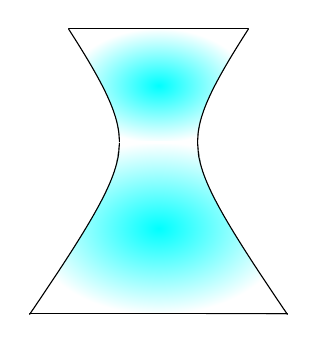
\begin{tikzpicture}[>=stealth,line join=round,line cap=round,font=\footnotesize,scale=.31,xscale=.8]
			\begin{scope}
				\fill[inner  color=cyan]
					 (-4.6,4.67)-- plot[domain=-4.6:-2] (\x,{1.12*((\x)^2-4)^0.5})--(2,0)
					 --plot[domain=2:4.6](\x,{1.12*((\x)^2-4)^0.5})--cycle;
				\fill[inner  color=cyan]
					(-6.6,-7)--  plot[domain=-6.6:-2] (\x,{-1.12*((\x)^2-4)^0.5})--(2,0)
					--plot[domain=2:6.6](\x,{-1.12*((\x)^2-4)^0.5})--cycle; 
				\fill[inner color=white]  (-2,1pt)--(-2,-1pt)--(2,-1pt)--(2,1pt)--cycle;
			\end{scope}
			 \clip (-6.7,-7.1) rectangle (6.7,4.7);
			 \draw[smooth,samples=100,domain=-4.6:-2] plot (\x,{1.12*((\x)^2-4)^0.5});
			 \draw[smooth,samples=100,domain=2:4.6] plot (\x,{1.12*((\x)^2-4)^0.5});
			\draw[smooth,samples=100,domain=-6.6:-2] plot  (\x,{-1.12*((\x)^2-4)^0.5});
			\draw[smooth,samples=100,domain=2:6.6]  plot (\x,{-1.12*((\x)^2-4)^0.5});
			\draw  (-6.6,-7)--(6.6,-7);
			\draw (-4.6,4.67)--(4.6,4.67); 
		\end{tikzpicture}
	 }
	 \shortans{125}
	\loigiai{ 
	\immini 
		{ 
		 Chọn hệ trục toạ độ $Oxy$ như hình vẽ.\\
		Phương trình chính  tắc của hypebol có dạng $\dfrac{x^2}{a^2}- \dfrac{y^2}{b^2}=1$.\\
		 Theo giả thiết ta có
		\begin{itemize}
			\item $F_1F_2=2c=20  \Rightarrow c=10$.
			\item $A_1A_2=2a=16 \Rightarrow  a=8$.
		\end{itemize}
		Suy ra $b=\sqrt{c^2-a^2}=6$.\\ 
		Do đó phương trình chính tắc của hypebol  là $\dfrac{x^2}{64}- \dfrac{y^2}{36}=1$.\\
		Gọi $R$ là bán kính đáy tháp,  $h$ là khoảng cách từ tâm đối xứng của hypebol đến đáy tháp.\\
		Ta  có $\pi R^2=10\,064\pi \Rightarrow R=4\sqrt{629}$ m.
		} 
		{ 
		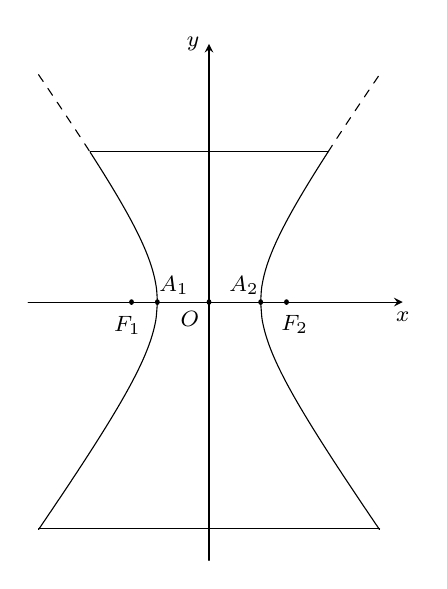
\begin{tikzpicture}[>=stealth,line join=round,line cap=round,font=\footnotesize,scale=.41,xscale=.8]
				\draw[->] (-7,0)--(7.5,0) node[below]  {$x$};
				\draw[->] (0,-8)--(0,8)  node[left] {$y$};
				\clip (-7,-8)  rectangle (7.5,8);
				\draw[smooth,samples=100,domain=-4.6:-2] plot (\x,{1.12*((\x)^2-4)^0.5}); 
				\draw[smooth,samples=100,domain=2:4.6] plot (\x,{1.12*((\x)^2-4)^0.5}); 
				 \draw[dashed,smooth,samples=100,domain=-6.6:-4.6] plot (\x,{1.12*((\x)^2-4)^0.5});
				\draw[dashed,smooth,samples=100,domain=4.6:6.6] plot (\x,{1.12*((\x)^2-4)^0.5}); 
				\draw[smooth,samples=100,domain=-6.6:-2] plot  (\x,{-1.12*((\x)^2-4)^0.5});
				\draw[smooth,samples=100,domain=2:6.6] plot (\x,{-1.12*((\x)^2-4)^0.5}); 
				\draw (-6.6,-7)--(6.6,-7); 
				\draw (-4.6,4.67)--(4.6,4.67); 
				\draw[fill=black] 
					 (-2,0) circle (2pt) node[shift=(45:3mm)] {$A_1$}
					 (2,0) circle (2pt) node[shift=(135:3mm)] {$A_2$}
					(-3,0) circle (2pt) node[shift=(-100:3mm)]  {$F_1$}
					(3,0)  circle (2pt) node[shift=(-70:3mm)] {$F_2$}
					 (0,0) circle (2pt) node[below left] {$O$};
			\end{tikzpicture}
		} 
		\noindent Thay $x=4\sqrt{629}$ vào phương trình $\dfrac{x^2}{64}- \dfrac{y^2}{36}=1$  ta tìm được $y=-75$, suy ra $h=75$.\\
		Theo đề bài ta có  chiều cao của tháp là $h+\dfrac{2}{3}h=75+\dfrac{2}{3}\cdot 75=125$ m.
	} 
\end{bt}


%%%%%%%%%%%%%%%% TỰ LUẬN %%%%%%%%%%%%%%%%

% nguồn: MaHoaNH_TuLuan_Lop10
\begin{bt}%[0H9V5-0]%[ma:11548309]
	 \immini{
	Một elip $(E)\colon \dfrac{x^2}{a^2}+\dfrac{y^2}{b^2}=1$, ($a>b>0$) với bán trục lớn $a$, bán tiêu cự $c$, thì tỉ số $e=\dfrac{c}{a}$ được gọi là tâm sai của elip. Quỹ đạo của trái đất quay quanh mặt trời là một elip $(E)$, trong đó mặt trời là một trong các tiêu điểm. Biết khoảng cách  nhỏ nhất và lớn nhất giữa mặt trời và trái đất lần lượt là $147$ triệu km và $152$ triệu km. Tâm sai của elip $(E)$ là $\dfrac{m}{n}$ (với $\dfrac{m}{n}$ là phân số tối giản). Tính $T=m+n$.
	 }
	{\begin{tikzpicture}[scale=1,font=\footnotesize,line join=round,line cap=round,>=stealth]
		 \def\xmin{-3.5}\def\xmax{3.5}\def\ymin{-2.5}\def\ymax{2.5}\pgfmathsetmacro\c{1.5}
		\clip (\xmin,\ymin)  rectangle (\xmax,\ymax);
		 \path
			 (-\c,0) coordinate (F_1)
			(1.5,1.6) coordinate (M); 
		 \draw [blue]
			(0,0) ellipse (2.5cm  and 2cm);
		\fill[blue]  (M) node[above right]{Trái đất} circle (2.5pt);
		\fill[red]  (F_1) node[below]{Mặt trời} circle (5pt);
	\end{tikzpicture}
	 }
	\loigiai{Elip có phương trình $(E)\colon \dfrac{x^2}{a^2}+\dfrac{y^2}{b^2}=1$, ($a>b>0$), $c=\sqrt{a^2-b^2}$.\\ 
		Khoảng cách từ một điểm $M$ bất kỳ thuộc elip có hoành  độ $x_M$ là $d_M=a\pm \dfrac{c\cdot x_M}{a}$, cho nên khoảng cách lớn nhất và nhỏ nhất từ một tiêu điểm đến $M$ lần lượt là $a+c$ và $a-c$.\\
		 Ta có hệ phương trình $\heva{&a+c=152\\&a-c=147}\Leftrightarrow \heva{&a=\dfrac{299}{2}\\&c=\dfrac{5}{2}.}$\\
		Vậy tâm sai của elip  $(E)$ là $e=\dfrac{c}{a}=\dfrac{5}{299}\Rightarrow \heva{&m=5\\& n=299}$ và $T=m+n=304$.
	 }
\end{bt}

% nguồn: MaHoaNH_TuLuan_Lop10
\begin{bt}%[0H9V5-0]%[ma:ad167802]
	Để chụp toàn cảnh, ta có thể sử dụng một gương hypebol. Máy ảnh được hướng về phía đỉnh của gương và tâm quang học của  máy ảnh được đặt tại một tiêu điểm của gương (xem hình). Tìm khoảng cách từ tâm quang của máy ảnh đến đỉnh của gương, biết rằng phương trình mặt cắt của gương là $\dfrac{x^2}{25}-\dfrac{y^2}{16}=1$.
	\begin{center}
		\begin{tikzpicture}[scale=0.6,font=\footnotesize,line join=round,line cap=round,>=stealth]
				\def\xmin{-10}\def\xmax{10}\def\ymin{-5}\def\ymax{5}\pgfmathsetmacro\c{2*sqrt  (5)}
				\draw[->] (\xmin-0.2,0)--(\xmax+0.2,0) node[below] {\footnotesize $x$}; 
				 \draw[->] (0,\ymin-0.2)--(0,\ymax+0.2) node[right] {$y$};
				\clip (\xmin,\ymin) rectangle (\xmax,\ymax); 
				 \path
					 (0,0) coordinate (O)
					(-2,0)  coordinate (A_1)
					(2,0) coordinate  (A_2)
					 (-\c,0) coordinate (F_1)
					(\c,0) coordinate (F_2) 
					 (-6.3,3) coordinate (M)
					(-6.3,-3) coordinate  (N);
				 \draw[blue] (M)--(N);
				\fill[blue!50]  (F_2) circle (0.3cm);
				\fill[blue!10]  (M)--(N)--plot ({-2*sqrt (\x*\x+1)},{\x})--(M);
				 \draw[smooth,variable=\x,blue] plot ({2*sqrt (\x*\x+1)},{\x});
				 \draw[smooth,variable=\x,blue] plot ({-2*sqrt (\x*\x+1)},{\x});
				\foreach \x/\g  in {F_1/-90,F_2/-90}
				\fill  (\x) circle (4.5pt);
				\foreach \x/\g  in {F_1/-90,F_2/-90,A_1/-40,A_2/240,O/-120}
				 \fill (\x) circle (1.5pt)
					 ($(\x)+(\g:7mm)$) node{$\x$};
				\draw (M)--($(M)+(30:1)$) node[above]{gương hypebol}; 
				\draw (F_2)--($(F_2)+(130:3)$) node[above]{tâm máy  ảnh};
				 \draw[dashed](A_1)--(F_1);
			\end{tikzpicture}
	\end{center}
	\loigiai{ Gọi $(H)\colon \dfrac{x^2}{25}-\dfrac{y^2}{16}=1\Rightarrow  \heva{&a^2=25\\&b^2=16}\Rightarrow \heva{&a=5\\&b=4}\Rightarrow c=\sqrt{a^2+b^2}=\sqrt{39}$.\\
		Tiêu điểm của  gương là $F_1\left(-\sqrt{39};0\right)$ và $F_2\left(\sqrt{39};0\right)$.\\
		Đỉnh của gương là  $A_1(-5;0)$.\\
		Vậy khoảng cách từ tâm của máy ảnh tới đỉnh của gương là\\  $F_2A_1=OA_1+OF_2=5+\sqrt{39}\approx 11{,}2$.
	} 
\end{bt}

% nguồn: MaHoaNH_TuLuan_Lop10
\begin{bt}%[0H9V5-0]%[ma:7edeadb1]
	Để cắt một bảng hiệu quảng cáo hình elip có  trục lớn bằng $80$ cm và trục nhỏ bẳng $40$ cm từ một tấm ván ép hình chữ nhật $ABCD$ có kích thước $80$ cm $40$ cm. Người ta vẽ hình elip đó lên tấm ván ép (như hình vẽ) bằng một vòng dây qua hai cái đinh ghim vào hai tiêu điểm. Hỏi phải lấy vòng dây có độ dài là bao nhiêu cm (làm tròn đến hàng đơn vị).
	\begin{center}
		\begin{tikzpicture}[scale=0.7,font=\footnotesize,line join=round,line cap=round,>=stealth]
				\def\xmin{-5}\def\xmax{5}\def\ymin{-3}\def\ymax{3}\pgfmathsetmacro\c{2*sqrt (3)} 
				\draw[->] (\xmin-0.2,0)--(\xmax+0.2,0) node[below] {\footnotesize $x$}; 
				\draw[->] (0,\ymin-0.2)--(0,\ymax+0.2)  node[right] {$y$};
				\draw (0,0) node [below left]  {$O$};
				\clip (\xmin,\ymin)  rectangle (\xmax,\ymax);
				 \path
					(-4,0) coordinate (A_1) node[below left]{$-a$} 
					 (4,0) coordinate (A_2) node[below right]{$a$}
					 (0,-2) coordinate (B_1) node[below left]{$-b$}
					(0,2)  coordinate (B_2) node[above left]{$b$}
					(-\c,0) coordinate  (F_1) node[above]{$-c$}
					 (\c,0) coordinate (F_2) node[above left]{$c$}
					(3,1.32)  coordinate (M)
					 (-4,2) coordinate (A)
					 (-4,-2) coordinate (D)
					(4,2) coordinate  (B)
					 (4,-2) coordinate (C);
				\draw 
					 (0,0) ellipse (4cm and 2cm)
					(A)--(B)--(C)--(D)--(A) 
					 (F_1)--(M)--(F_2)--cycle;
				\fill (M) node[above]{$M$} circle (1.5pt); 
				\foreach \x/\g  in {F_1/-90,F_2/-90,A/135,B/45,C/-45,D/-135}
				\fill (\x)  circle (1.5pt)
					 ($(\x)+(\g:4mm)$) node{$\x$};
			\end{tikzpicture}
	\end{center}
	 \loigiai{
		Ta có $\heva{&2a=80\\& 2b=40}\Leftrightarrow \heva{&a=40\\&b=20}$. 
		Khi đó $c=\sqrt{a^2-b^2}=20\sqrt{3}$. 
		\begin{itemize}
			\item Tiêu điểm $F_1(-20\sqrt{3};0)$ và $F_2(20\sqrt{3};0)$.\\ 
			Do đó hai đinh cách  mép tấm ván là $F_1A_1=F_2A_2=40-20\sqrt{3}\approx 5{,}36$ cm.
			\item  Đỉnh $B_2(0;40)$.
			 \item $MF_1=\sqrt{(20\sqrt{3})^2+40^2}=20\sqrt{7}$ cm.
			\item Vòng dây có độ dài $F_1F_2+MF_1+MF_2=40\sqrt{3}+40\sqrt{7}\approx 175$  cm.
		\end{itemize}
	 }
\end{bt}
